\documentclass[
    author={Jacob Daniel Halsey},
    supervisor={Prof. Awais Rashid},
    degree={BSc},
    title={Building a Testbed for Evaluating Privacy Enhancing Technologies  (PETs)},
    subtitle={},
    type={software development},
    year={2021}
]{dissertation}

\usepackage[backend=biber,bibstyle=ieee,citestyle=numeric]{biblatex}
\bibliography{dissertation}

\usepackage{setspace} 
\setstretch{1.25}

\usepackage{subfig}

\usepackage{listings, listings-rust}
\lstset{
	frame=tb,
	language=Rust,
	keywordstyle=\color{blue},
	stringstyle=\color{code-string},
	commentstyle=\color{code-comment},
	tabsize=4,
	basicstyle={\small\ttfamily},
	showstringspaces=false,
	breaklines=true,
	aboveskip=3mm,
	belowskip=0mm,
}

\usepackage{nameref}

\begin{document}

\maketitle
\frontmatter
\makedecl
\tableofcontents

\chapter*{Executive Summary}

The goal of this project is to produce a simple and lightweight testbed platform for evaluating privacy enhancing
technologies.
It should provide support for testing varied architectures and network topologies, such as client-server and
peer-to-peer applications.
It should also support simulating applications for different types of platforms including mobile phone apps.

\vspace{1cm}

Summary of work:

\begin{itemize}
\item I have developed a flexible command line tool called \emph{kvm-compose} for Linux using the Rust
      language and \emph{libvirt} library for building and destroying virtual testing environments.
\item In the process I have made some contributions to open source libraries including \texttt{libvirt-rust}
(the \emph{Rust} language bindings to \emph{libvirt}).
\item I have then implemented some example projects using the testbed tool.
\end{itemize}

\chapter*{Supporting Technologies}
\label{chap:supporting_tech}

\begin{singlespace}
	\begin{itemize}
		\item \emph{Linux KVM} (Kernel-based Virtual Machine) - \url{https://www.linux-kvm.org/}
		\item \emph{Open vSwitch} Virtual multilayer switch - \url{https://www.openvswitch.org/}
		\item \emph{libvirt} Virtualization API - \url{https://libvirt.org/}
		\item \emph{Rust} Language, Compiler, Toolchain, etc. - \url{https://www.rust-lang.org/}
		\item \emph{libvirt-rust} Rust bindings to the libvirt - \url{https://gitlab.com/libvirt/libvirt-rust}
		\item \emph{clap} Rust command Line Argument Parser - \url{https://github.com/clap-rs/clap}
		\item \emph{serde} Rust Serialization framework - \url{https://github.com/serde-rs/}
		\item \emph{serde-yaml} YAML backend for serde - \url{https://github.com/dtolnay/serde-yaml}
		\item \emph{serde-plain} Plain text backend for serde - \url{https://github.com/mitsuhiko/serde-plain}
		\item \emph{thiserror} Rust error derive macro - \url{https://github.com/dtolnay/thiserror}
		\item \emph{anyhow} Rust error handling framework - \url{https://github.com/dtolnay/anyhow}
		\item \emph{simple\_logger} Rust logging implementation - \url{https://github.com/borntyping/rust-simple_logger}
		\item \emph{xml-rs} XML library for Rust - \url{https://github.com/netvl/xml-rs}
		\item \emph{validator} Rust struct validation - \url{https://github.com/Keats/validator}
		\item \emph{directories} User data directories library - \url{https://github.com/dirs-dev/directories-rs}
		\item \emph{reqwest} Rust HTTP Client - \url{https://github.com/seanmonstar/reqwest}
		\item \emph{indicatif} Rust command line progress indicator - \url{https://github.com/mitsuhiko/indicatif}
		\item \emph{tempfile} Rust temporary file library - \url{https://github.com/Stebalien/tempfile}
		\item \emph{casual} Rust user input parser - \url{https://github.com/rossmacarthur/casual}
		\item \emph{derive-new} Rust new constructor macro - \url{https://github.com/nrc/derive-new}
		\item \emph{enum-iterator} Rust macro for iterating enums - \url{https://github.com/stephaneyfx/enum-iterator}
		\item \emph{rust-embed} Embeds files into Rust binaries - \url{https://github.com/pyros2097/rust-embed}
	\end{itemize}
\end{singlespace}

\chapter*{Acknowledgements}

I would like to thank my supervisor Professor Awais Rashid and co-supervisor Joe Gardiner for their
project proposal and support and guidance in completing it.

\mainmatter


\chapter{Contextual Background}
\label{chap:context}

The UK Research and Innovation (UKRI) is a non-departmental public body of the United Kingdom Government
sponsored by the Department for Business, Energy and Industrial Strategy~\cite{ukri_who_we_are}.
In October 2020 the UKRI announced the creation of the National Research Centre on Privacy, Harm Reduction
and Adversarial Influence Online (REPHRAIN)~\cite{ukri_new_centre}.
The centre is made up of researchers in computer science, international relations, law, psychology, management,
design, digital humanities, public policy, political Science, criminology, and sociology from five British
universities including the University of Bristol. \\

REPHRAIN should be understood in the context of the UK government's \emph{Online Harms White Paper} public
consultation beginning in April 2019~\cite{uk_gov_online_harms}, which sets out plans for new online safety 
measures; REPHRAIN's missions and outcomes are aligned with this paper~\cite{rephrain_harms}. \\

REPHRAIN will focus on three core missions~\cite{rephrain_missions}:

\begin{enumerate}
	\item Delivering privacy at scale while mitigating its misuse to inflict harms.
	\item Minimising harms while maximising benefits from a sharing-driven digital economy.
	\item Balancing individual agency vs. the social good.
\end{enumerate}

The three missions will require looking at Privacy Enhancing Technologies (PETs); including their capabilities,
applications of PETs in addressing existing online harms, mitigating the potential abuse of PETs, embedding the PETs
into infrastructures, and developing new PETs.
In order to facilitate this REPHRAIN intends to build a toolbox of resources including a PETs testbed. The testbed
will be used by researchers in developing, testing, and evaluating the PETs. 
The aim of this project is to develop a prototype for this testbed.

\section{What are Privacy Enhancing Technologies (PETs)?}

Before we discuss Privacy Enhancing Technologies we must consider what we mean by "privacy". REPHRAIN is 
primarily using the definitions set out by D. J. Solove in his
2006 article \emph{A Taxonomy of Privacy}~\cites{solove_privacy}{rephrain_harms}. Solove notes that the
definition of privacy has often been very broad or vague, and therefore sets out to develop
a taxonomy of privacy violations. He has defined four groups of harmful activities (See figure~\ref{privacy_taxonomy}). \\

\begin{figure}
\centering
\parbox{7cm}{
	\begin{enumerate}
		\item Information collection
		\begin{enumerate}
			\item Surveillance
			\item Interrogation 
		\end{enumerate}
		\item Information processing
		\begin{enumerate}
			\item Aggregation
			\item Identification
			\item Insecurity
			\item Secondary Use
			\item Exclusion
		\end{enumerate}
	\end{enumerate}
}
\qquad
	\begin{minipage}{7cm}
		\begin{enumerate}
			\setcounter{enumi}{2}
			\item Information  dissemination
			\begin{enumerate}
				\item Breach of Confidentiality
				\item Disclosure
				\item Exposure
				\item Increased Accessibility
				\item Blackmail
				\item Appropriation
				\item Distortion
			\end{enumerate}
			\item Invasion
			\begin{enumerate}
				\item Intrusion
				\item Decisional Interference
			\end{enumerate} 
		\end{enumerate}
	\end{minipage}
	\caption{A Taxonomy of Privacy Violations~\cite{solove_privacy}.}
	\label{privacy_taxonomy}
\end{figure}

Broadly speaking a Privacy Enhancing Technology is any solution or approach in hardware or software that helps
protect a user from such privacy violations~\cite{buckley_pets}. Some examples of PETs could include 
Onion routing such as the Tor network (which enables anonymous communication), or
end-to-end encrypted messaging systems such as the Signal protocol. 
Kaaniche et al.~\cite{kaaniche_2020_privacy} have defined a more comprehensive classification of PETs
 (see Figure~\ref{pet_taxonomy}).

\begin{figure}
	\centering
	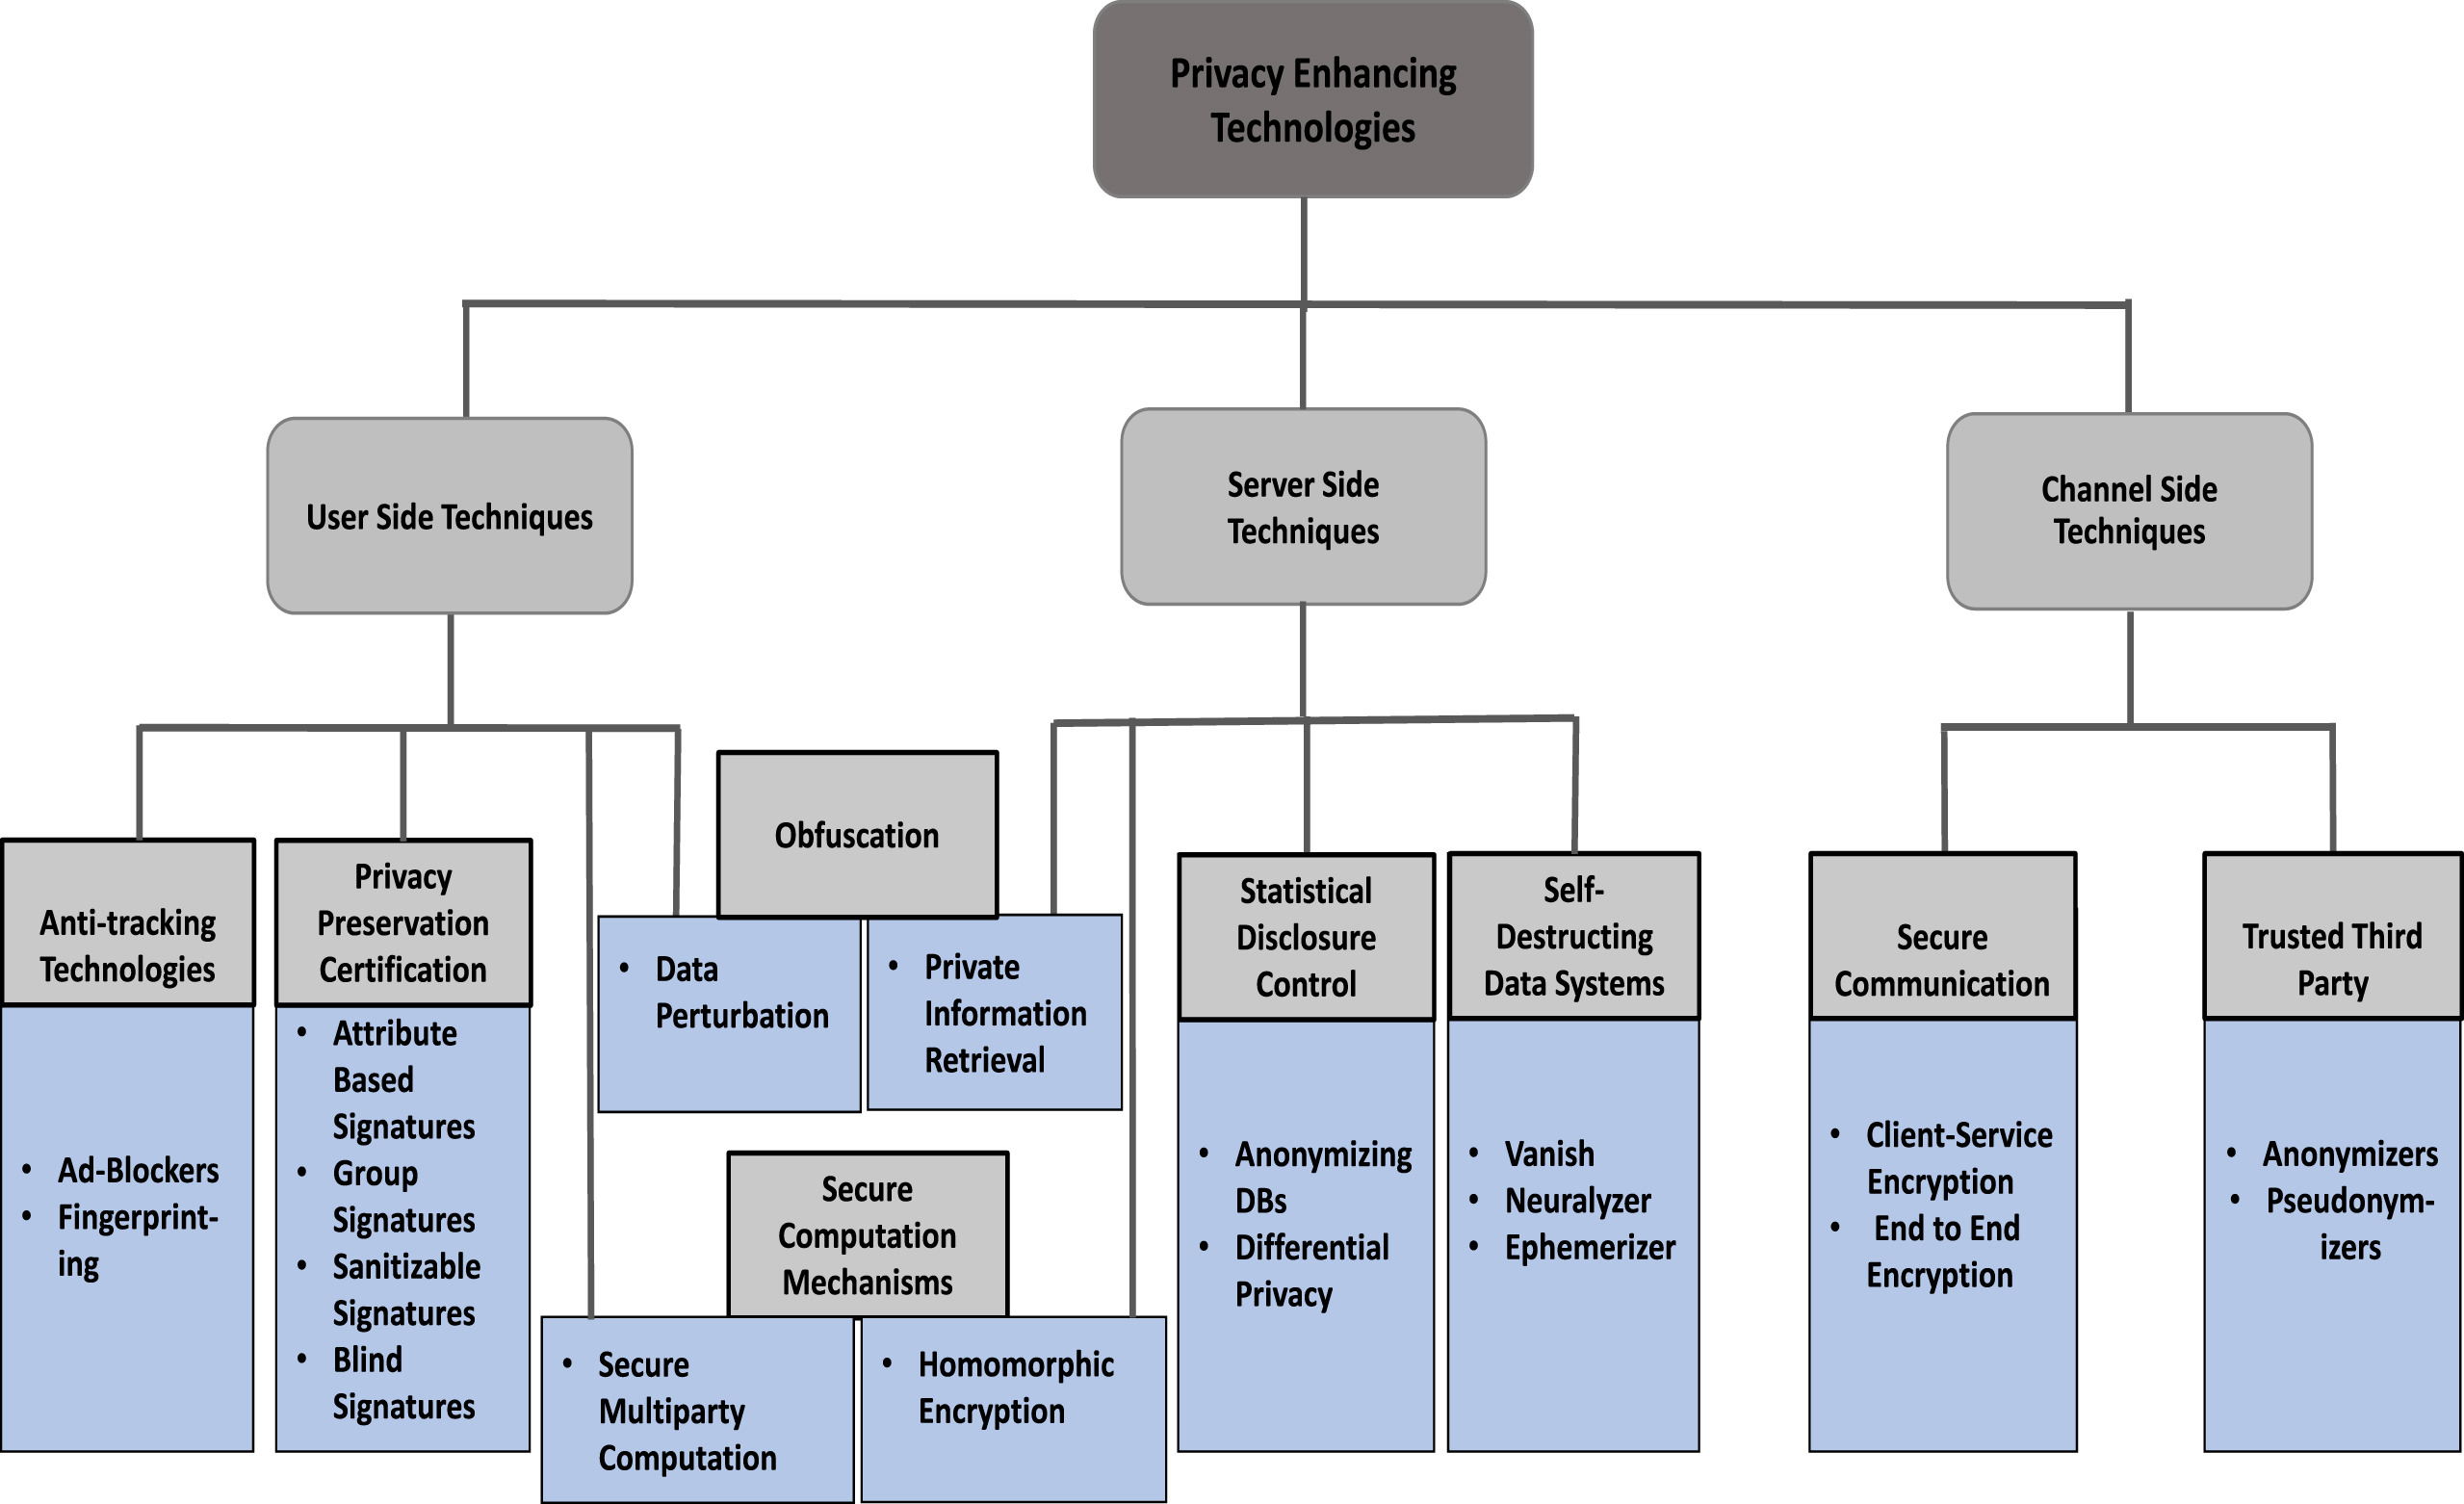
\includegraphics{img/pet_taxonomy}
	\caption{A Taxonomy of privacy enhancing technologies~\cite{kaaniche_2020_privacy}.}
	\label{pet_taxonomy}
\end{figure}

\section{Existing Solutions}

There has been some existing research by Tekeoglu and Tosun~\cite{tekeoglu_2016_testbed} who have developed 
a privacy testbed for Internet-of-Things (IoT) devices. Their approach has some similar goals to this project 
in that it looks at capturing layer 2 and 3 network traffic. They note that the testbed enables experiments such
as port vulnerability scans, checking what cipher suites are used (or not), and generally monitoring 
network traffic to see what data is being collected. However their testbed is different in that it is only designed
for IoT devices; rather than general purpose PET applications.

\section{High Level Objectives}

Overall the high-level objective of this project is to develop a simple and lightweight
testbed platform for evaluating PETs:

\begin{itemize}
	\item The testbed should support testing various architectures and network topologies, 
	including client/server and peer-to-peer applications, to accommodate a variety of PETs.
	\item The testbed should be able to collect information such as packet captures
	for use in evaluating the privacy properties.
	\item The testbed should support different platforms such as desktop and mobile apps,
	and both applications where the source code is available or only pre-built binaries.
	\item The testbed should enable a high level of automation, such that working with large test
	environments because feasible, and the setup can easily and programmatically be replicated.
\end{itemize}

\chapter{Technical Background}
\label{chap:technical}

In this chapter I will discuss some of the technologies which this project depends or builds upon.

\section{Virtualization}

\begin{quotation}
	`Virtualization uses software to create an abstraction layer over computer hardware that allows the hardware 
	elements of a single computer—processors, memory, storage and more—to be divided into multiple virtual computers, 
	commonly called virtual machines (VMs). Each VM runs its own operating system (OS) and behaves like an independent 
	computer, even though it is running on just a portion of the actual underlying computer hardware.'~\cite{ibm_virtualization}
\end{quotation}

Virtualization\footnote{I am a British citizen, and this is a dissertation at a British university, 
and therefore I am very much aware that the correct spelling in British English is `virtualisation', however the
majority of platforms, libraries, and sources I will be referencing use the US English spelling, 
so I have chosen to do the same. Likewise the same applies for `containerization'.}
 will therefore be a very useful technology for the testbed, since it will allow us to model
an environment consisting of multiple computers such as application clients and servers, and run
them all within a single machine. In addition, modern CPU extensions (such as \emph{Intel VT} and \emph{AMD-V}) 
provide hardware-assisted / accelerated virtualization support, allowing the virtual machines to 
have near native performance which will help in meeting the goal of minimal overhead for the testbed. \\

In order to use virtualization a \emph{Hypervisor} is required, this is the software layer sits between
the physical hardware and manages the virtual machines. A hypervisor may run directly on the physical machine
in place of a conventional operating system - as a Type 1 or \emph{bare-metal} hypervisor,
or run within a separate host operating system - as a Type 2 or \emph{hosted} hypervisor. \\

\subsection{\emph{KVM}}
\label{subsect:kvm}

For the prototype testbed I will be using \emph{Kernel-based Virtual Machine} (KVM), which is a 
kernel module for the Linux operating system that allows it to function as a hypervisor. 
The advantage is that \emph{KVM} (and the Linux kernel itself) are free and open-source software 
under GNU licenses, and it is a stable and mature platform~\cite{redhat_kvm}.
In userspace \emph{QEMU}\footnote{Note \emph{QEMU} can also function as its own independent type 2 hypervisor 
	but \emph{KVM} is required to enable hardware acceleration,
see \url{https://www.packetflow.co.uk/what-is-the-difference-between-qemu-and-kvm/}}
may then use KVM to provide a full virtualization platform. \\

\emph{libvirt} is an open-source toolkit for managing virtualization platforms~\cite{libvirt},
it supports \emph{QEMU/KVM} as well as hypervisors from other vendors. It is written in C, 
with bindings available in many other programming languages, making it a suitable library for developing 
the testbed. Support for other platforms also means it would be easier to add support
for additional hypervisors in future.

\section{Containerization}
\label{sect:containerization}

Having discussed full platform / machine virtualization it is worth also mentioning containerization
which is an alternative lightweight approach to virtualizing applications. In particular 
there is the Docker platform for Linux containers which has become very popular in recent
years~\cite{zdnet_docker_2018}. \\

\begin{figure}
	\centering
	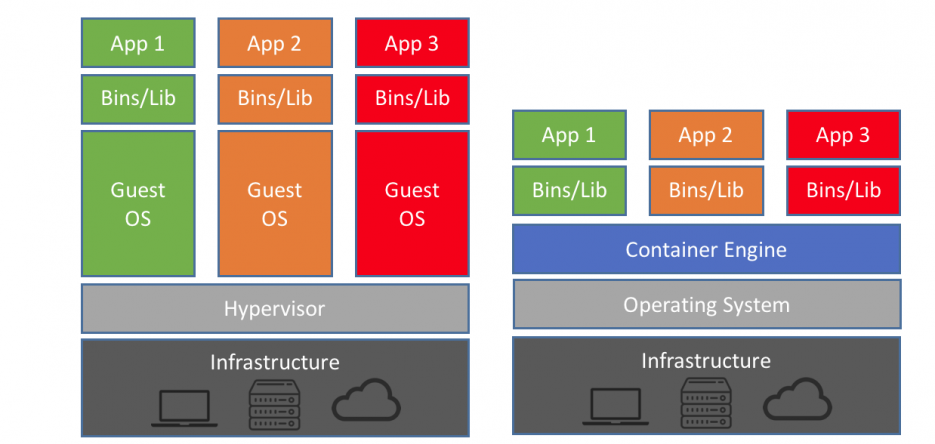
\includegraphics[width=12cm]{img/containers}
	\caption[]{Platform Virtualization vs Containerization\footnotemark}
	\label{containers_diagram}
\end{figure}
\footnotetext{Graphic from \url{https://blog.netapp.com/blogs/containers-vs-vms/}}

Unlike full platform virtualization, containerization does not virtualize a whole computer 
(or require hardware acceleration), instead it uses namespacing within the host operating 
system kernel to create an isolated environment. This has many practical uses, making deploying
software and services very quick and easy, but unfortunately it is not ideal for our testbed, since
it would mean all applications would have to use the same operating system; it couldn't be 
used to simulate different platforms. \\

While I will not be using containerization, the \emph{Docker Compose} tool~\cite{docker_compose}
used for orchestrating containers has provided some useful inspiration for the testbed.
\emph{Docker Compose} is a command line program with two core subcommands \emph{up}
and \emph{down} which are used to either build or destroy a set of containers as defined
in a YAML configuration file. The configuration file may define a list of containers, each 
with options including an image to download, an entry command to run, volumes to attach,
and environment variables, the config may also define virtual networks and attach them
to the containers. These are all very useful features in line with the goals for the testbed, and as such
I will try to replicate them but within a fully virtualized environment (\emph{QEMU/KVM}).

\section{Virtual Networks}

Once we have created virtual machines, a hypervisor needs the ability to bridge traffic between
the virtual machines and the external network~\cite{openvswitch_why}. 
One method of doing of doing so with \emph{QEMU/KVM} is to use the 
\emph{Linux Bridge}\footnote{\url{https://wiki.linuxfoundation.org/networking/bridge}},
this is a virtual layer 2 switch built into the \emph{Linux} kernel, that can be
managed with the \texttt{bridge-utils} package (or equivalent). \\

There is also an alternative virtual networking solution for \emph{Linux} (and other platforms)
- \emph{Open vSwitch}. The advantages of \emph{Open vSwitch} over \emph{Linux Bridge} include that it has
easy management via SDN (explained below), it can support more complex network protocols, and it can
function as a Layer 3 router (as opposed to just a Layer 2 bridge).

\subsection{Software Defined Networking (SDN)}

In order to understand Software Defined Networking (SDN) we must first explain how networking
devices such as switches and routers function. 

The \emph{data plane} refers to the functions of a network device that actually process and forward
packets between interfaces. For example the ASIC (application specific integrated circuit) logic
that matches packets to a routing table.

The \emph{control plane} refers to the processes that a network device uses in order to control
the data plane; to determine which paths a particular packet should take. For example a
dynamic routing protocol such as OSPF that programs a routing table.

The \emph{management plane} refers to the protocols that a network administrator can
use to manage and configure the network device. For example the SSH protocol can be used
to remotely connect a console.

SDN refers to the practice of removing the control plane responsibilities of each individual
network device, and centralising the control plane within an 
SDN controller~\cite[760]{odom_2016_ccna}.\\

\begin{figure}
	\centering
	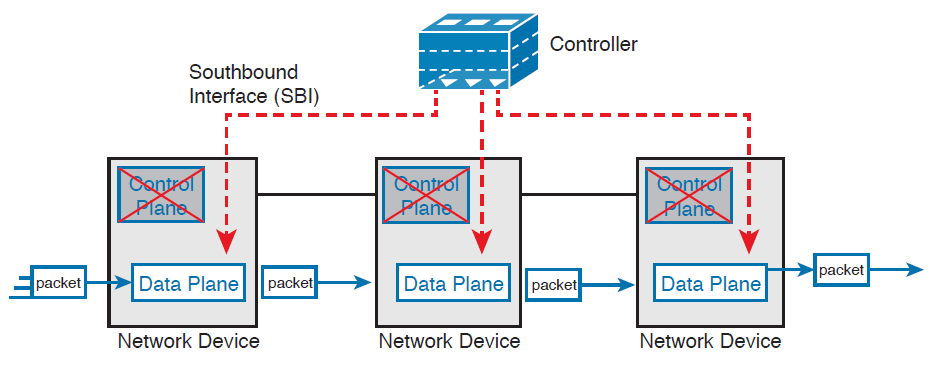
\includegraphics[width=12cm]{img/sdn}
	\caption{Use of an SDN controller~\cite[767]{odom_2016_ccna}}
	\label{fig:sdn_diagram}
\end{figure}

The benefit of SDN is that it can simplify network management since the network can be 
managed from a single controller. This is especially useful in this scenario of 
a virtual testbed because researchers are likely to want to be able to quickly conduct experiments 
varying the structure of the virtual network while testing PETs.\\

\emph{OpenFlow} is a protocol that implements SDN by allowing remote access / control to the data plane
of a switch or router~\cite{openflow}. \emph{OpenFlow} is supported by \emph{Open vSwitch}, and there
are a number of free and open-source SDN controllers that also support \emph{OpenFlow} such as
\emph{Floodlight}\footnote{\url{https://floodlight.atlassian.net/wiki/spaces/floodlightcontroller/overview}}
and \emph{OpenDaylight} (ODL)\footnote{\url{https://www.opendaylight.org/}}.

\section{The Rust Language}

As you will see in Chapter~\ref{chap:execution}, I have chosen to use the Rust programming
language for developing the testbed. Although there are no doubt many languages which
could have been used, I will provide some background on Rust, and its advantages for this
project. \\

Rust is a modern systems programming language, originally developed by Mozilla, 
with its first stable release in 2015. It is designed with a focus on performance, safety
and concurrency. \\

\begin{singlespace}
	It has some key advantages:
	\begin{itemize}
		\item Excellent performance; on par with
		 \emph{C/C++}\footnote{\url{https://benchmarksgame-team.pages.debian.net/benchmarksgame/index.html}}.
		\item Easy interaction with \emph{C} libraries via FFI, making 
		the \emph{libvirt}~\cite{libvirt_rust} bindings possible.
		\item A simple to use package manager - \emph{Cargo},
		along with a rich ecosystem\footnote{\url{https://crates.io/}} of 
		libraries / crates\footnote{Rust packages 
			managed through the \emph{Cargo} package
				manager are known as \emph{Crates}}.
		\item Modern functional constructs such as sum types and pattern matching.
		\item Memory and thread safety are enforced at compile time~\cite{systems_rust}.
		\item The compiler and standard library support a large number of platforms.
	\end{itemize}
\end{singlespace}

\section{\emph{cloud-init}}
\label{sect:cloud-init-background}

One of the goals of the project is to support a high level of automation when building a 
test environment. So far we have looked at technologies we can use to create virtual machines,
but that would still leave the tester with a lot of work in terms of installing the operating
systems and software on the virtual machines. \\

One approach the tester could take is pre-building a machine step by step,
installing all their software and configuring it appropriately, and then saving
a disk image, which they could attach to virtual test machines. However that approach 
has some weaknesses; first of all if they wish to change on of the earlier steps
such as their choice of operating system it would require starting the process from scratch,
another problem is that each clone of the disk image would be the same, and customisation
would require manually logging in to each individual instance.
Also if the tester wants to transfer or replicate the testbed it would mean copying
a series of potentially large disk images with duplicate data. \\

The problem of automatically initialising virtual machines is not unique to this testbed project,
in fact it is shared by public cloud providers (such as \emph{Amazon AWS}, \emph{Microsoft Azure},
\emph{Oracle OCI}, etc.), who need to deploy various operating systems (of many different versions)
and then configure them so the customer can remotely connect.
As a result a standard system for initialising cloud machines has
been developed called \emph{cloud-init}~\cite{cloud_init} - which has support for many popular operating systems,
cloud platforms and data sources. \\

It works by having a \emph{cloud-init} package already installed as part of the operating system,
in a `cloud image', usually available directly from the operating system maintainers
\footnote{For example \url{https://cloud-images.ubuntu.com/}}.
On the first boot of the image \emph{cloud-init} will check for supported data sources,
(such as from a list of supported URLs) from which to obtain user data and instance meta data.
The data can include things such locale, hostname, and SSH keys which are then automatically
applied to the instance.

\chapter{Project Execution}
\label{chap:execution}

\section{\emph{kvm-compose}}

To provide the core functionality of the testbed I have developed a command line tool called \emph{kvm-compose},
using the technologies described in chapter \ref{chap:technical}, namely \emph{QEMU/KVM}, 
\emph{libvirt}, \emph{Open vSwitch}, \emph{cloud-init}, and the \emph{Rust} language.

\subsection{Dependencies and Installation}
\label{sect:dependencies}

In order to compile the project it requires the \emph{Rust} compiler\footnote{\url{https://www.rust-lang.org/tools/install}},
and the \texttt{libvirt-dev} and \texttt{libssl-dev} packages (or system equivalent).
The \emph{bash} script \texttt{kvm-compose/install.sh} may be used to compile \emph{kvm-compose},
install the binary into a system folder, and change its ownership to \emph{root}.
Note that the \emph{root} permission is added so that the utiltiy may access \texttt{qemu:///system}
and modify the \emph{Open vSwitch} and other networking configurations. \\

To successfully use \emph{kvm-compose} the following packages should be installed (or equivalent):
\texttt{qemu-kvm libvirt-daemon-system libvirt-clients openvswitch-switch}. Hardware acceleration
for virtualization should be enabled in the system, and if required for the application being tested - 
nested virtualization for KVM should also be 
enabled\footnote{\url{https://docs.fedoraproject.org/en-US/quick-docs/using-nested-virtualization-in-kvm/}}.

\subsection{Command Line Interface (CLI)}

As mentioned in section \ref{sect:containerization} the CLI is partly inspired by \emph{docker-compose}.
It has two main subcommands \texttt{up} and \texttt{down} which create or destroy a testbed environment.
It will look for a configuration file called \texttt{kvm-compose.yaml} in the current directory (unless
otherwise specified with the \texttt{--input} flag).
And the current directory name is taken to be used as the `project name' (again unless specified with
the \texttt{--project-name} flag). The \emph{clap} crate was used to automatically parse the command line arguments
in a type-safe manner. \\ 

The basic principle for the \texttt{up} command is to first iterate over all the configured network bridges,
if each bridge does not already exist it is then created as per the configuration, with the project name as a prefix.
The prefix is used to reduce the possibility that resources in the current testbed project will conflict
with other existing configuration on the system or other testbed projects. 
After creating the bridges it then iterates over all the configured virtual machines, if it does not exist
it is created according to its specification (with the project prefix) and then launched. 
Files required for the virtual machines to function such as disk images are placed in the current directory.
The \texttt{down} command does the opposite in reverse order;
stopping and removing the machines (and any left over files), and then removing the bridges. \\

There is also the \texttt{machine} subcommand which can be used to \texttt{up} or \texttt{down} individual machines
without affecting the rest of the testbed, in the event the user wishes to just make configuration changes
to a small number of virtual machines.

\begin{figure}
	\begin{verbatim}
		kvm-compose 1.0
		Jacob Halsey
		
		USAGE:
		kvm-compose [FLAGS] [OPTIONS] <SUBCOMMAND>
		
		FLAGS:
		-h, --help       Prints help information
		--no-ask     Suppress (accept) continue prompts
		-V, --version    Prints version information
		
		OPTIONS:
		--input <input>                  Configuration file [default: kvm-compose.yaml]
		--project-name <project-name>    Defaults to the current folder name
		-v, --verbosity <verbosity>          
		
		SUBCOMMANDS:
		cloud-images    List supported cloud images
		down            Destroy all virtual devices in the current configuration
		help            Prints this message or the help of the given subcommand(s)
		machine         Configure individual machine
		up              Create all virtual devices in the current configuration
	\end{verbatim}
	\caption{\emph{kvm-compose} usage / help output}
	\label{fig:kvm_compose_usage}
\end{figure}

\subsection{Configuration File Format}

The configuration file is expected to be in the YAML format~\cite{yaml}, internally \emph{kvm-compose}
uses the \emph{serde} and \emph{serde-yaml} crates to parse the file.
The root of the config file should look like:

\begin{verbatim}
machines:                       # List of testbed virtual machines
bridges:                        # List of testbed virtual bridges
ssh_public_key: ssh-rsa...      # Your SSH public key
\end{verbatim}

An example machine config could look like:

\begin{verbatim}
- name: example1                # (VM will be prefixed with project name)
  memory_mb: 4096               # Optional: default 512MiB
  cpus: 4                       # Optional: default 1
  disk:                         # Two variants: cloud_image or existing_disk 
    cloud_image:
      name: ubuntu_18_04
      expand_gigabytes: 25      # Optional: Adds additional space to the virtual disk
  interfaces:                   # List of connected network interfaces
    - bridge: br0               # (A bridge defined in the same project)
  run_script: ./script.sh       # Optional: path to a script
  context: ./file.txt           # Optional: path to a file or folder
  environment:                  # Dictionary of arbitary environment variables
    key: value                  # Use /etc/nocloud/env.sh *key* to query
\end{verbatim}

Alternatively an existing disk image may be used instead of a cloud image:

\begin{verbatim}
    existing_disk:
      path: ./disk.img         # Path to the disk image
      driver_type: qcow2       # raw or qcow2 (Default: raw)
      device_type: disk        # disk or cdrom (Default: disk)
      readonly: false          # Default: false
\end{verbatim}


Assuming that the disk image supports \emph{cloud-init}\footnote{
	\emph{cirros-init} is also supported but only when used with the \emph{cirros} cloud image
} at first boot the following will happen:

\begin{singlespace}
	\begin{itemize}
		\item The machine \texttt{name} (with project prefix) is used as the hostname.
		\item The SSH public key is injected into the instance.
		\item File(s) specified in \texttt{context} are copied into the \texttt{/etc/nocloud/context} directory.
		\item The \texttt{run\_script} is executed, with its output log saved into \texttt{/etc/nocloud/}.
	\end{itemize}
\end{singlespace}

An example virtual bridge config could look like:

\begin{verbatim}
- name: br0                     # (Bridge will be prefixed with project name)
      # Optionally connect to a physical interface on the host
      # Such as to allow the virtual machines internet access
  connect_external_interfaces: [eth0]
      # When 'stealing' one of the host's adapters 
      # you will need to assign the new virtual adapter an IP
  enable_dhcp_client: true
      # Optional: Specify an SDN controller to use
  controller: tcp:127.0.0.1:6653
      # Optional: Specify which protocol to use for the SDN controller
  protocol: OpenFlow13
\end{verbatim}

\subsection{Interaction with \emph{QEMU/KVM}}

I have used the \emph{libvirt} library for interacting with \emph{QEMU/KVM}, 
via the bindings to access it from the \emph{Rust} language: \emph{libvirt-rust}~\cite{libvirt_rust}.
One of the benefits of the \emph{kvm-compose} tool is that it automates the creation of \emph{libvirt Domain}
XML configurations (with the help of the \emph{xml-rs} crate). These are otherwise tedious to write, for 
example it generates the following XML to send to \emph{libvirt}:

\begin{verbatim}
<?xml version="1.0" encoding="UTF-8"?>
<domain type="kvm">
  <name>signal-client1</name>
  <cpu mode="host-model" />
  <vcpu>2</vcpu>
  <memory unit="MiB">2048</memory>
  <os>
    <type arch="x86_64">hvm</type>
  </os>
  <devices>
    <graphics type="vnc" port="-1" autoport="yes" />
    <disk type="file" device="disk">
      <driver name="qemu" type="qcow2" />
      <source file="/home/jacob/independent-project/examples/signal/client1-cloud-disk.img" />
      <target dev="hda" bus="ide" />
    </disk>
    <disk type="file" device="cdrom">
      <driver name="qemu" type="raw" />
      <source file="/home/jacob/independent-project/examples/signal/client1-cloud-init.iso" />
      <readonly />
      <target dev="hdb" bus="ide" />
    </disk>
    <interface type="bridge">
      <source bridge="signal-br0" />
      <virtualport type="openvswitch" />
    </interface>
  </devices>
  <sysinfo type="smbios">
    <system>
      <entry name="serial">ds=nocloud;</entry>
    </system>
  </sysinfo>
</domain>
\end{verbatim}

\subsection{Modifications to \emph{libvirt-rust}}

During my early work developing the project I discovered that under certain build setups / toolchains
the \emph{libvirt-rust} crate
failed to compile, due to it containing function declarations that did not actually exist in the \emph{libvirt}
library. This is described in full detail in my issue
report: \url{https://gitlab.com/libvirt/libvirt-rust/-/issues/1}.\\

I submitted a fixed version of \emph{libvirt-rust} with these invalid functions removed, but also with
a test case that builds the bindings in a static library, therefore checking that all the symbols (such as
functions) did actually exist in the underlying \emph{libvirt} library. 
The tests are automatically run as part of the 
CI/CD pipeline so this sort of problem should be prevented in future. The merge request was approved by
the project maintainers: \url{https://gitlab.com/libvirt/libvirt-rust/-/merge_requests/14}. \\

Whilst working with \emph{libirt} I also discovered that I was receiving duplicate error messages printed
to the console (via \emph{stdout/stderr}), this was because by default \emph{libvirt} has an error handler
configured to print all errors, but at the same time the \emph{libvirt-rust} binding functions also returned
a \lstinline|Result<_, virt::error::Error>| type (the idiomatic approach in Rust), 
which on failure I was also printing to the console
via the logging framework. So I also added a \lstinline|clear_error_func()| to the merge request
that binds to \lstinline|virSetErrorFunc| so that the default error handler can be disabled.

\subsection{Cloud Images}

The currently supported cloud images may be listed using the \texttt{cloud-images} subcommand 
of \emph{kvm-compose}. When a cloud image is chosen and launched \emph{kvm-compose} takes the following
steps:

\begin{singlespace}
	\begin{enumerate}
		\item Checks if the image has already been downloaded, the \texttt{directories} crate 
		is used to resolve the path (\texttt{\$HOME/.kvm-compose/} on Linux).
		\item If not it will prompt the user before downloading; the download may be large so it makes sense
		to check first (this behaviour can be disabled with the \texttt{--no-ask} option for use in
		an unattended script). \texttt{Reqwest} is used for the download along with the \texttt{indicatif}
		crate to display progress.
		\item A copy of the image with the machine name will be made in the current directory.
		\item The disk image will be expanded if the \texttt{expand\_gigabytes} option is specified.
		\item The disk is attached to virtual machine via the \emph{libvirt Domain} XML.
	\end{enumerate}
\end{singlespace}

\subsection{\emph{cloud-init}}

Section \ref{sect:cloud-init-background} provides an introduction to \emph{cloud-init}, but I
will now explain how it has been used in \emph{kvm-compose}.
When a virtual machine is created the virtual bios is configured to use the string
\texttt{ds=nocloud} in the serial number. This indicates to \emph{cloud-init} that 
the \texttt{NoCloud} datasource\footnote{\url{https://cloudinit.readthedocs.io/en/latest/topics/datasources/nocloud.html}}
is being used. On startup the \emph{cloud-init} agent will then look for an \emph{ISO9660/Joliet} or \emph{vfat}
filesystem with a volume label of \texttt{cidata}. \\

When creating virtal machines \emph{kvm-compose} calls the \texttt{genisoimage} program\footnote{\url{https://linux.die.net/man/1/genisoimage}}
to generate a \emph{Joliet} filesystem containing a \emph{cloud-init} user data and instance metadata file.
The instance metadata is a JSON encoded file; on \texttt{NoCloud} this can contain an automatically configured
hostname, as well as any other keys. 
The keys also accessible via the \texttt{cloud-init query ds.meta\_data.*key*} command inside the VM.
The user data is a \texttt{\#cloud-config} file in the YAML format, which when loaded by the \emph{cloud-init}
agent it is put through the \emph{jinja} templating engine, allowing variable substitution from the instance
metadata values\footnote{See \texttt{/kvm-compose/assets/cloud\_init.yaml}, the file is embedded in the binary
using the \texttt{rust-embed} crate.}.
The context file(s) are made available to the virtual machine as a \emph{tarball} in the same \emph{Joliet} volume.
The \texttt{\#cloud-config} file is used to list a number of startup commands
necessary to provide the features
needed by \emph{kvm-compose} - such as launching and logging the \texttt{run\_script} and extracting in
the \texttt{context} file(s) to the local disk.\\

\emph{kvm-compose} also supports the \emph{Cirros} cloud image - this is a minimal Linux distribution
by the \emph{OpenStack Project}\footnote{\url{https://docs.openstack.org/image-guide/obtain-images.html\#cirros-test}}.
I have added support because due to its small footprint it could be useful when launching a large 
number of virtual machines on a resource constrained system.
Note that when using \emph{Cirros} the \emph{cloud-init} setup works slightly differently because \emph{Cirros}
does not have a full \emph{cloud-init} implementation - instead it uses \emph{cirros-init} which doesn't support
\texttt{\#cloud-config}; the user data can only be a simple 
script\footnote{See \texttt{/kvm-compose/assets/cirros\_init.sh}}.
Instance metadata keys are instead accessed via \texttt{cirros-query get *key*} command.

\section{Examples}

I have provided two example projects demonstrating how \emph{kvm-compose} can be used to automatically
create a virtual testbed environment for privacy enhancing technologies (PETs).

\subsection{\emph{DP3T}}

Decentralized Privacy-Preserving Proximity Tracing (\emph{DP3T}) is an open protocol developed for
digital contact tracing during the COVID-19 pandemic, originating from the École polytechnique fédérale 
de Lausanne (EPFL) and ETH Zurich, it was developed with the intention of being less centralised
than alternative solutions, and therefore more private~\cite{busvine_2020}. 
Switzerland's national contact tracing app \emph{SwissCovid} 
has been built using the \emph{DP3T} protocol~\cite{swisscovid}. \\

The files in \texttt{/examples/dp3t} demonstrate how \emph{kvm-compose} can be used to build
a test environment. First of all a virtual machine for the backend service is defined,
which has a \texttt{run\_script} that on launch:

\begin{singlespace}
	\begin{enumerate}
		\item Installs dependencies \emph{Git} and \emph{Maven}.
		\item Clones and builds the 
		\texttt{dp3t-sdk-backend}\footnote{\url{https://github.com/DP-3T/dp3t-sdk-backend}}.
		\item Installs and runs \emph{dp3t} as a service.
		\item Configures the network address of the server\footnote{
			Unfortunately \emph{Anbox} (discussed below) does not support using hostnames / DNS from 
			the host machine's network, so a static address has been used.}.
	\end{enumerate}
\end{singlespace}

\subsubsection{\emph{Android} App}

The \emph{DP3T} project provides an SDK (Software Development Kit) 
for both \emph{Android} and \emph{Apple iOS} which
is used to communicate with the backend server, it is this library which is used in the official
implementations such as \emph{SwissCovid}. The SDK also has a demo \texttt{calibration-app} (that uses
the SDK library) with a simple user interface of diagnostic tools and info, for use in testing the 
system\footnote{\url{https://github.com/DP-3T/dp3t-sdk-android/tree/master/calibration-app}}.
The \texttt{/examples/dp3t} contains a small patch to the source of the \texttt{calibration-app} that
changes the server URL to the backend in the testbed (as well as setting the correct keys). \\

\begin{figure}
	\centering
	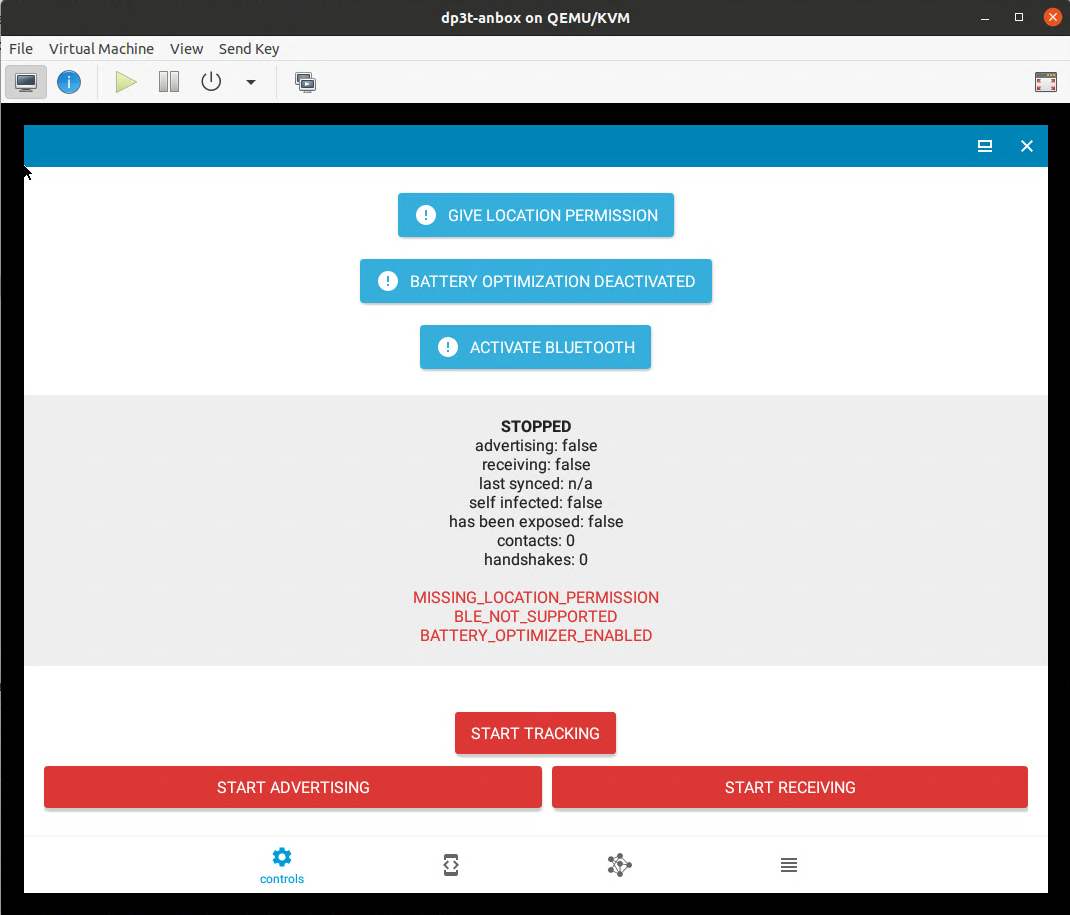
\includegraphics[width=13.5cm]{img/anbox}
	\caption{\emph{DP3T} \texttt{calibration-app} running in \emph{Anbox} on the testbed}
	\label{fig:anbox}
\end{figure}

\begin{figure}
	\centering
	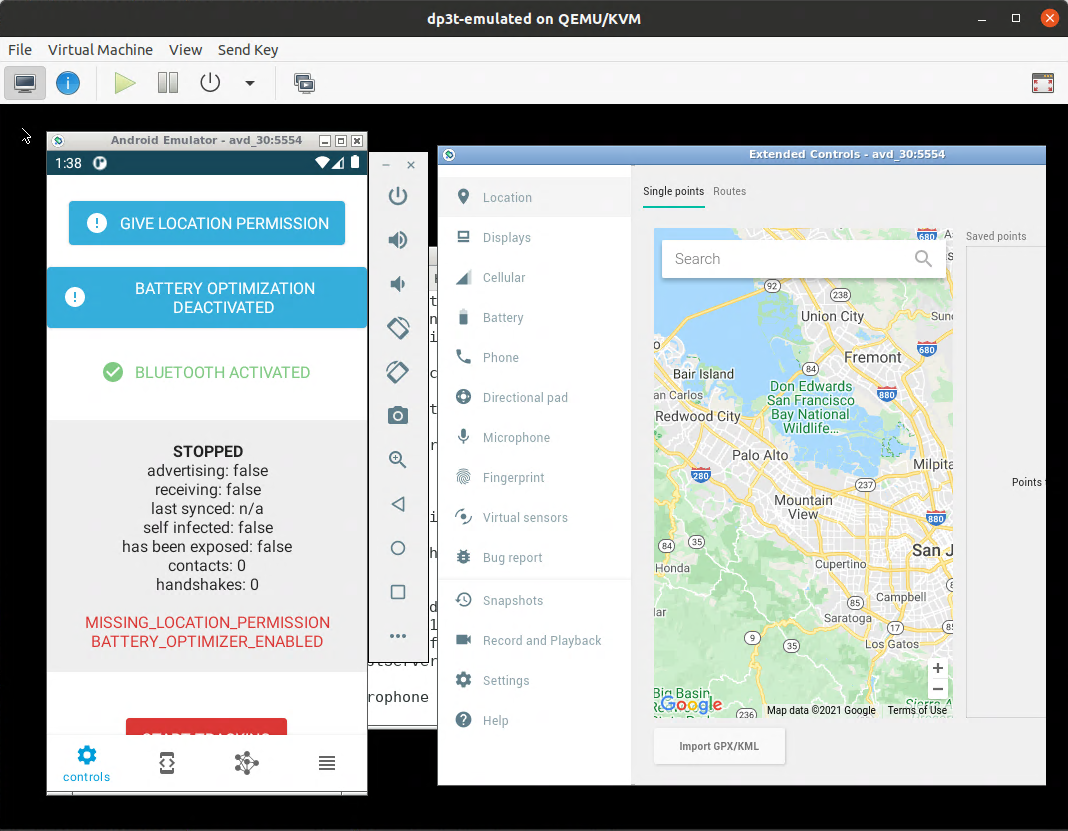
\includegraphics[width=13.5cm]{img/android_emulator}
	\caption{\emph{DP3T} \texttt{calibration-app} running in \emph{Android Emulator} on the testbed}
	\label{fig:anbox}
\end{figure}

To run the \texttt{calibration-app} I have provided two different example machines. The first
uses \emph{Anbox} which is a compatibility layer for running \emph{Android} apps within a \emph{Linux}
container\footnote{\url{https://anbox.io/}}, and the second uses the \emph{Android Emulator} 
(from the official \emph{Android SDK} / 
\emph{Android Studio})\footnote{\url{https://developer.android.com/studio/run/emulator}}
which uses full virtualization instead\footnote{It therefore requires nested 
virtualization to be enabled, see section \ref{sect:dependencies}.}.
For each of the two machines their \texttt{run\_script} installs the
dependencies and simulators. The \texttt{calibration-app} is made available in the machine in the 
\texttt{/etc/nocloud/context} folder, ready to be launched and used by the tester.
I chose to provide two \emph{Android} examples because each of the emulators have different
strengths and weaknesses; the \emph{Android Emulator} has more support for customising sensor
input such as GPS data, but it has poorer performance due to the extra layer of virtualization
when compared to \emph{Anbox}.

\subsection{\emph{Signal}}

\emph{Signal} is a messaging service built using its own custom end-to-end encryption protocol 
(the \emph{Signal Protocol}), available for a number of platforms on mobile and desktop,
designed with a focus on privacy~\cite{signal}. The standard service uses a central server
hosted and maintained by the \emph{Signal Foundation},
however the server code is also available under an open source 
license\footnote{\url{https://github.com/signalapp/Signal-Server}}. \\

The files in \texttt{/examples/signal} demonstrate how \emph{kvm-compose} can be used to build
a test environment. First of all a virtual machine for the signal server is defined,
which has a \texttt{run\_script} that on launch:

\begin{singlespace}
	\begin{enumerate}
		\item Installs dependencies \emph{Git}, \emph{Maven}, \emph{Docker} etc.
		\item Clones and builds the \emph{Signal} server.
		\item Launches a number of dependent services (\emph{Redis}, \emph{Postgres}, \emph{Nginx})
		in \emph{Docker} containers.
		\item Initialises the databases.
		\item Installs and runs the \emph{Signal} server as a service; configuration files
		are provided via \emph{kvm-compose}'s \texttt{context} option.
	\end{enumerate}
\end{singlespace}

The Signal server's configuration has test device numbers defined, allowing them
to be registered without requiring phone number verification.
The \emph{kvm-compose} configuration file then defines client 
machines using a \texttt{run\_script} that:

\begin{singlespace}
	\begin{enumerate}
		\item Installs dependencies \emph{Git} and \emph{Java}.
		\item Clones and builds \texttt{signal-cli}\footnote{\url{https://github.com/AsamK/signal-cli}}
		which is an open source command line wrapper around the \emph{Signal} SDK / client libraries.
		\item Before building, applies a small patch to change the server address to the hostname of the 
		\emph{Signal} server within the testbed. 
	\end{enumerate}
\end{singlespace}

When the client's \emph{Signal} server URL is patched, an \lstinline[language=java]|okhttp3.ConnectionSpec|
is also provided allowing cleartext (non HTTPS) communication between the client and server. This is useful
because it allows inspection of the packets which would otherwise be TLS encrypted. Unfortunately this 
exposed a bug in \texttt{libsignal-service-java} (a dependency of \texttt{signal-cli}) where the given
\lstinline[language=java]|ConnectionSpec| is only respected for RESTful but not WebSocket communications
with the \emph{Signal} server. I have submitted a pull request to fix this: \url{https://github.com/Turasa/libsignal-service-java/pull/28} which has since been merged.

\begin{figure}
	\centering
	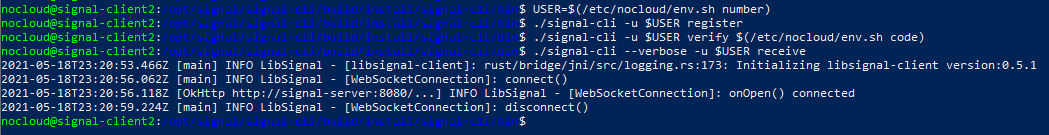
\includegraphics[width=16cm]{img/signal-cli}
	\caption{\texttt{signal-cli} registering and connecting via WebSockets to the testbed server}
	\label{fig:signal_cli}
\end{figure}

\subsection{Capturing Traffic}

When a test environment has been built (using the \texttt{kvm-compose up} command), network
traffic can then be collected using the \texttt{ovs-tcpdump} utlity of 
\emph{Open vSwitch}\footnote{\url{https://docs.openvswitch.org/en/latest/ref/ovs-tcpdump.8/}}.
For example:

\begin{verbatim}
	sudo ovs-tcpdump --span -i dp3t-br0 -w output.pcap
\end{verbatim}

The \texttt{-i} option is where the bridge name is specified, in the format of the project name
and bridge name (from the \texttt{kvm-compose.yaml} file) joined with a hyphen.
What this does is create a temporary mirror port on the specified bridge, with the \texttt{--span}
option indicating that traffic from all bridge ports should be mirrored. The output is saved as a
packet capture file which may be opened with software such as 
\emph{Wireshark}\footnote{\url{https://www.wireshark.org/}}.

\section{Development Practices}

During development I used the \emph{Git} version control system, with free hosting from \emph{GitHub Inc},
a \texttt{.gitignore} file was used to prevent temporary and user specific files being added to the
repository.
The \emph{IntelliJ Rust} plugin for \emph{CLion} proved very useful for code completion and other typical
IDE features\footnote{\url{https://www.jetbrains.com/rust/}}.
I also made use of the \emph{GitHub Actions} CI/CD platform, with a workflow configured to check that
the project builds and passes style checks on each push to the repository\footnote{See 
\texttt{.github/workflows/rust.yml}}. 

\chapter{Critical Evaluation}
\label{chap:evaluation}

\section{Results}


\section{REPHRAIN Feedback}

\section{Explanation of Failure Cases}


\section{Difficulties with Example Projects}

\subsection{\emph{NHS} COVID App and Cloud Lock-In}

Before creating the \emph{DP3T} example project I was originally intending to test the UK's \emph{NHS} COVID-19 
contact tracing app implementation\footnote{\url{https://github.com/nihp-public/covid19-app-system-public}}. 
However it quickly became apparent that the service is highly coupled to
\emph{Amazon Web Services (AWS)}, and as such it is very difficult to run within the testbed.
It is architectured using the serverless model, and depends on services includes using \emph{Amazon}'s 
\emph{API Gateway}, \emph{Lambda}, \emph{DynamoDB} etc.
Whilst it is indeed possible to run some of the \emph{AWS} services 
locally\footnote{For example: \url{https://hub.docker.com/r/amazon/dynamodb-local/}}, replicating
the entire \emph{AWS} infrastructure to simulate the COVID service would require a very substantial amount of 
time and effort; requiring code and configuration changes to enable connecting to local endpoints rather than the
\emph{AWS} regions.\\

This can be considered part of a broader problem of vendor lock-in in the context of modern
cloud services; due to a lack of standardization and unique cloud service implementations, it means
that applications are being developed that target a specific cloud service, and are not easy to move
without incurring engineering costs~\cite{cloud_lock_in}. This proves a challenge to the whole concept 
of a local virtual testbed in a world where technologies are being developed for specific proprietary
cloud services, without support for self hosting. As such to test them locally would require code modifications,
and the more the code is modified from the original, the less accurate and useful any test results can be 
considered, when compared to the real service.

\begin{figure}
	\centering
	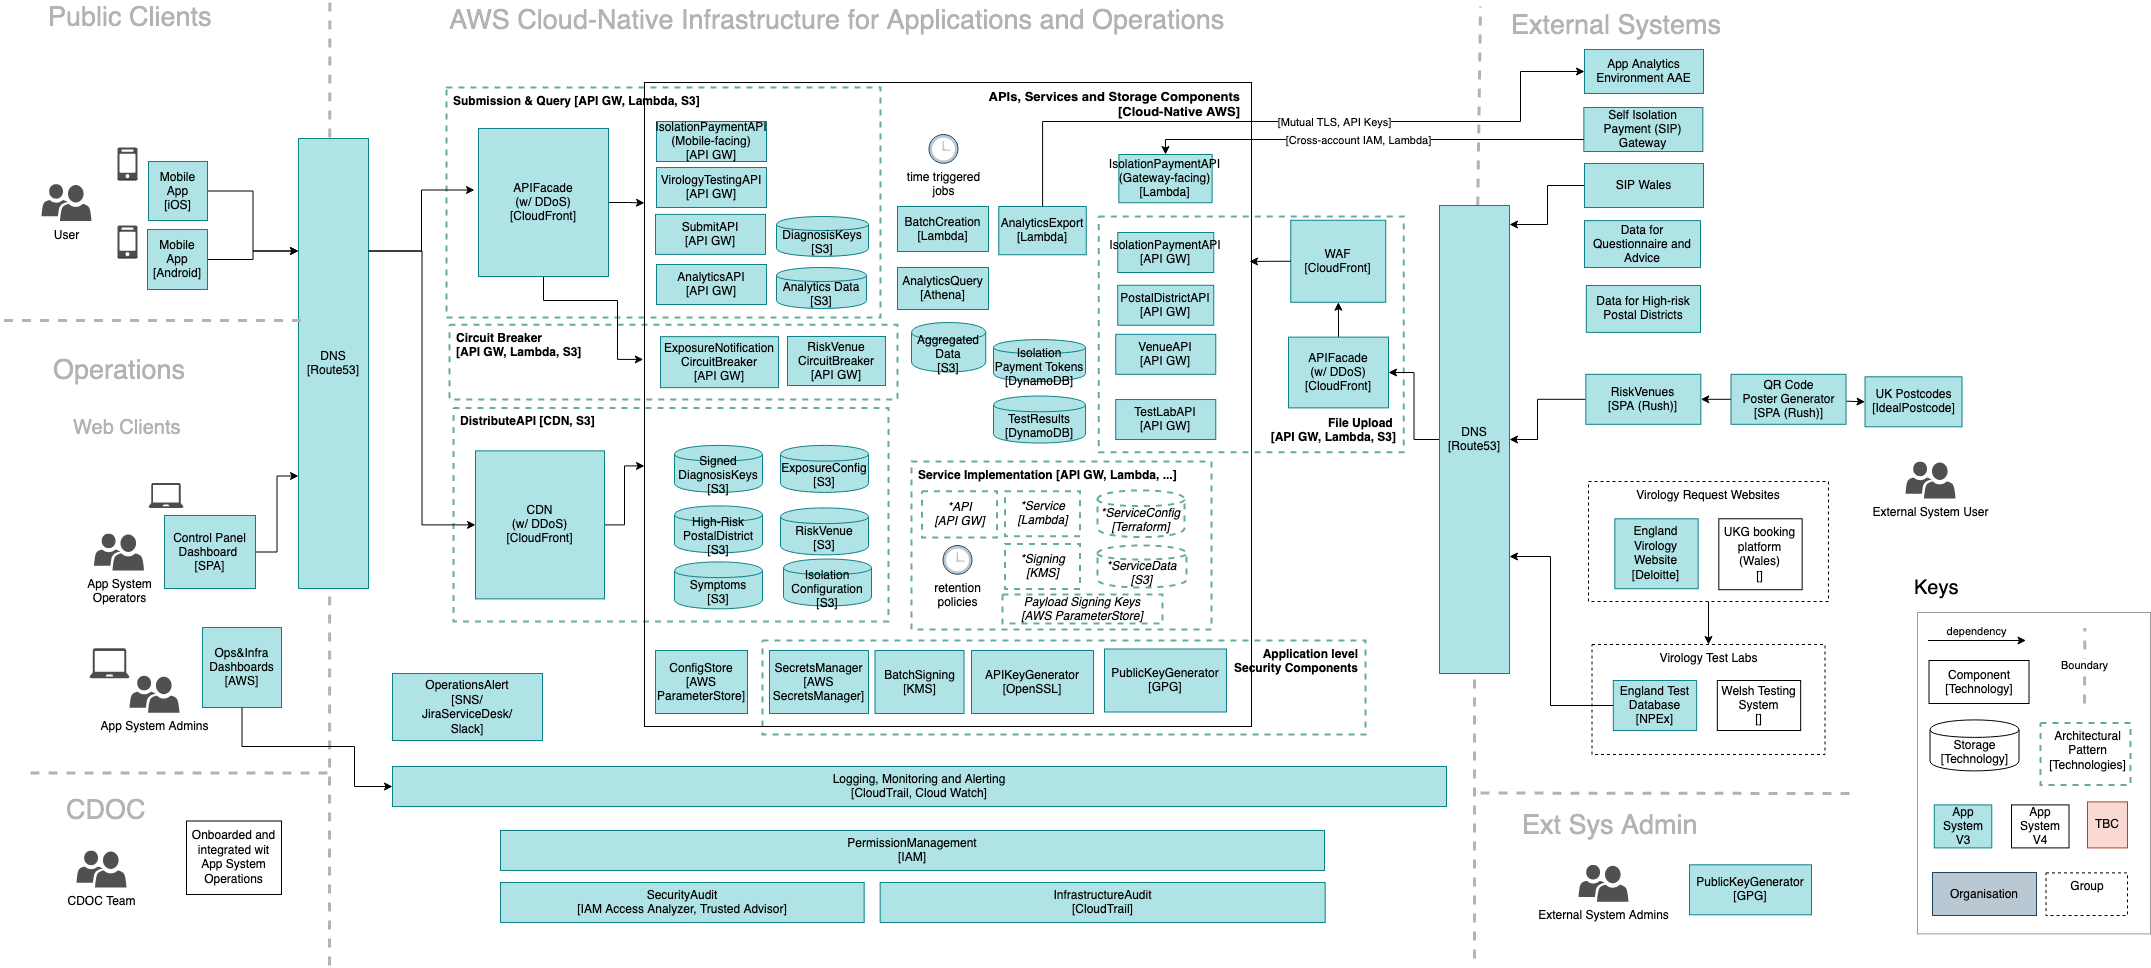
\includegraphics[width=16cm]{img/nhs-covid}
	\caption{\texttt{NHS} COVID-19 App System Architecture}
\end{figure}

\subsection{Exposure Notifications API}

After switching to the \emph{DP3T} service I was able to setup the backend server within
the testbed relatively easily, since it is implemented as a stand alone Spring Boot 
application\footnote{\url{https://spring.io/projects/spring-boot}}. However when attempting
to deploy the mobile client I then discovered another issue: in order to 
use the \emph{DP3T} \texttt{calibration-app}
it is required to enable the debug mode for COVID-19 exposure notifications within the
Android device settings, however that option was not available, since according to \emph{Google}:

\begin{quotation}
	To enable debug mode on a device, the primary account on the device must be a development account that is on the allowlist.\footnote{\url{https://developers.google.com/android/exposure-notifications/debug-mode}}
\end{quotation}

Allowlist membership is only available to government health authorities, and
official implementations of the app are distributed through \emph{Google}'s \emph{Play Store} and are
digitally signed, hence allowing them to make use of the exposure notification API. But these are not useful
for our testing purposes because we need to be able to change the URL to our own server. There does not
currently appear to be any method of using the API for debugging or testing 
purposes\footnote{\url{https://github.com/google/exposure-notifications-android/issues/8}}, meaning it cannot
be used within the testbed.\\

As a workaround for my example project so that I could demonstrate the \emph{DP3T} service being used,
I am using the \texttt{prestandard} edition, which used its own exposure detection protocol prior to the development
of the Google one\footnote{\url{https://github.com/DP-3T/dp3t-sdk-android\#introduction}}. 
Whilst this does allows the app to launch successfully and data to be collected in the testbed
it is no longer an accurate representation of the technology that is actually in live use. This highlights another
similar issue with the testbed concept, in that despite being designed with a focus on privacy and security~\cite{gaen}
some applications have been engineered without the ability to use in a test environment.




\subsection{\emph{Signal} Server}


\section{to do}

\begin{itemize}
	\item Show the testbed working, with packet trace data
	\item Signal v5 AWS dependency,  is difficult to test
	\item Signal setup documentation difficulties.
	\item rephrain meeting feedback
	\item talk about future improvements / additional features
\end{itemize}

\vspace{2cm} 
{\bf A topic-specific chapter, of roughly $15$ pages} 
\vspace{1cm} 

\noindent
This chapter is intended to evaluate what you did.  The content is highly 
topic-specific, but for many projects will have flavours of the following:

\begin{enumerate}
\item functional  testing, including analysis and explanation of failure 
      cases,
\item behavioural testing, often including analysis of any results that 
      draw some form of conclusion wrt. the aims and objectives,
      and
\item evaluation of options and decisions within the project, and/or a
      comparison with alternatives.
\end{enumerate}

\noindent
This chapter often acts to differentiate project quality: even if the work
completed is of a high technical quality, critical yet objective evaluation 
and comparison of the outcomes is crucial.  In essence, the reader wants to
learn something, so the worst examples amount to simple statements of fact 
(e.g., ``graph X shows the result is Y''); the best examples are analytical 
and exploratory (e.g., ``graph X shows the result is Y, which means Z; this 
contradicts [1], which may be because I use a different assumption'').  As 
such, both positive {\em and} negative outcomes are valid {\em if} presented 
in a suitable manner.

\chapter{Conclusion}
\label{chap:conclusion}

{\bf A compulsory chapter,     of roughly $5$ pages} 
\vspace{1cm} 

\noindent
The concluding chapter of a dissertation is often underutilised because it 
is too often left too close to the deadline: it is important to allocation
enough attention.  Ideally, the chapter will consist of three parts:

\begin{enumerate}
\item (Re)summarise the main contributions and achievements, in essence
      summing up the content.
\item Clearly state the current project status (e.g., ``X is working, Y 
      is not'') and evaluate what has been achieved with respect to the 
      initial aims and objectives (e.g., ``I completed aim X outlined 
      previously, the evidence for this is within Chapter Y'').  There 
      is no problem including aims which were not completed, but it is 
      important to evaluate and/or justify why this is the case.
\item Outline any open problems or future plans.  Rather than treat this
      only as an exercise in what you {\em could} have done given more 
      time, try to focus on any unexplored options or interesting outcomes
      (e.g., ``my experiment for X gave counter-intuitive results, this 
      could be because Y and would form an interesting area for further 
      study'' or ``users found feature Z of my software difficult to use,
      which is obvious in hindsight but not during at design stage; to 
      resolve this, I could clearly apply the technique of Smith [7]'').
\end{enumerate}

\backmatter
\printbibliography

\end{document}
